\begin{figure}[htbp]
\centering
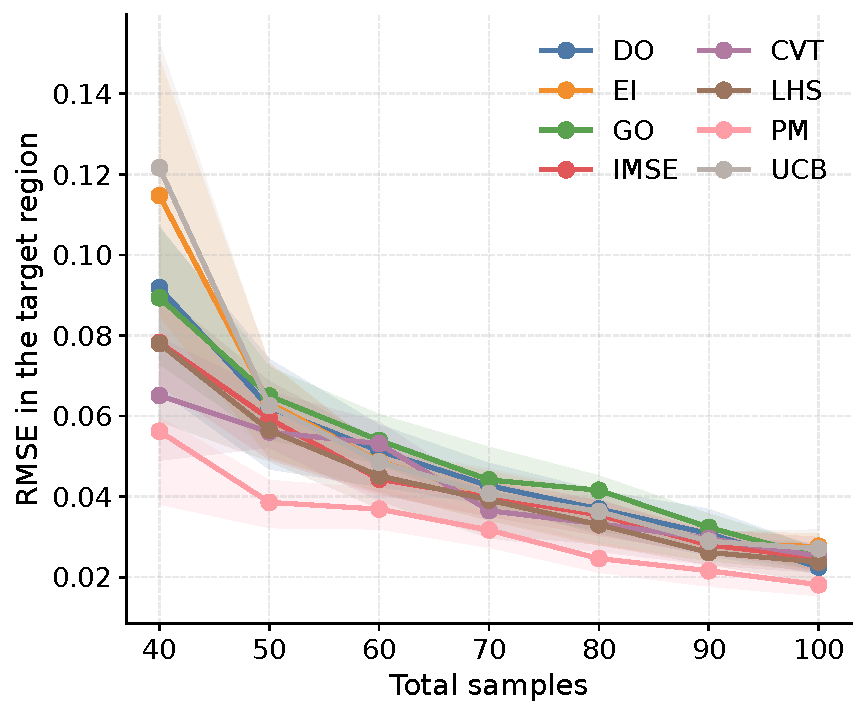
\includegraphics[width=\linewidth]{2d_target_10.pdf}
\caption{RMSE in the target region for the 2D example with 10 active learning points.}
\label{fig:sub_2d_target_10}
\end{figure}

\begin{figure}[htbp]
\centering
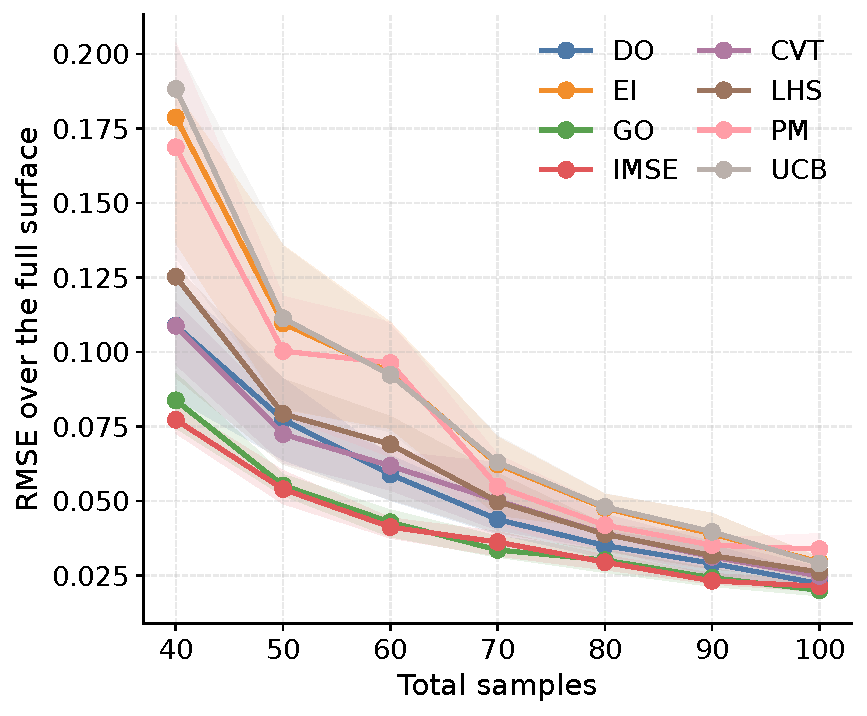
\includegraphics[width=\linewidth]{2d_overall_10.pdf}
\caption{RMSE over the full surface for the 2D example with 10 active learning points.}
\label{fig:sub_2d_overall_10}
\end{figure}

\begin{figure}[htbp]
\centering
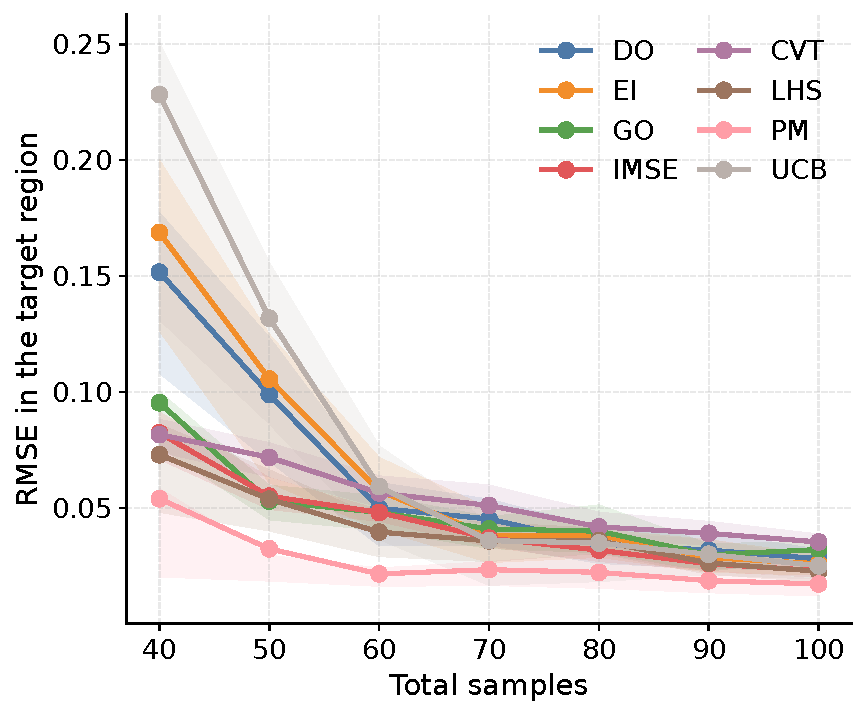
\includegraphics[width=\linewidth]{2d_target_20.pdf}
\caption{RMSE in the target region for the 2D example with 20 active learning points.}
\label{fig:sub_2d_target_20}
\end{figure}

\begin{figure}[htbp]
\centering
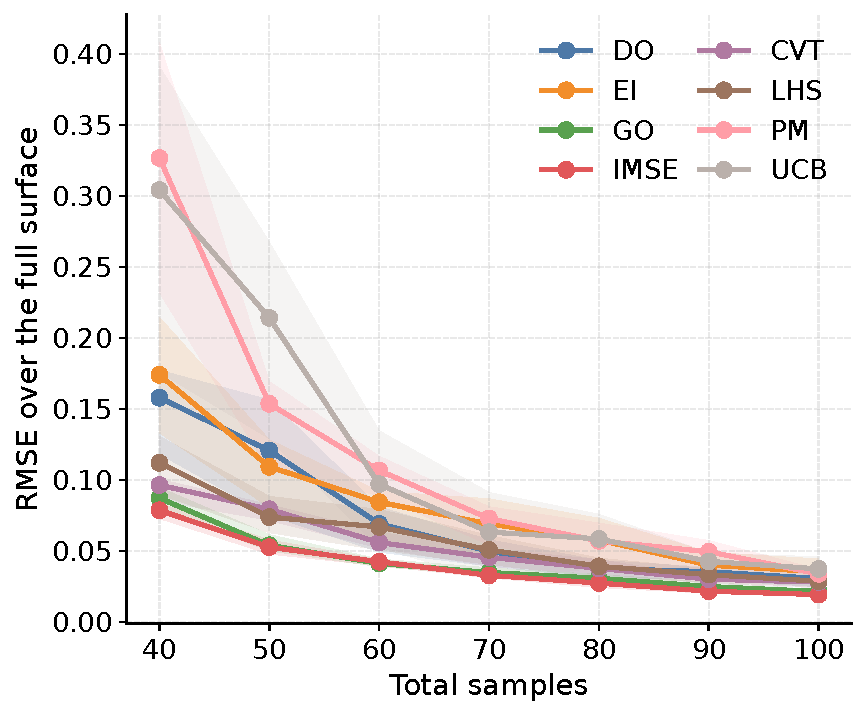
\includegraphics[width=\linewidth]{2d_overall_20.pdf}
\caption{RMSE over the full surface for the 2D example with 20 active learning points.}
\label{fig:sub_2d_overall_20}
\end{figure}
